% По умолчанию используется шрифт 14 размера. Если нужен 12-й шрифт, уберите опцию [14pt]
%\documentclass[14pt]{matmex-diploma}
\documentclass[14pt]{matmex-diploma-custom}

\begin{document}
% Год, город, название университета и факультета предопределены,
% но можно и поменять.
% Если англоязычная титульная страница не нужна, то ее можно просто удалить.
\filltitle{ru}{
    chair              = {Программная инженерия\\Системное программирование},
    title              = {Универсальный механизм первичного поиска повторов в тексте для пакета Duplicate Finder},
    % Здесь указывается тип работы. Возможные значения:
    %   coursework - Курсовая работа
    %   diploma - Диплом специалиста
    %   master - Диплом магистра
    %   bachelor - Диплом бакалавра
    type               = {master},
    position           = {студента},
    group              = 21.М07-мм,
    author             = {Глазырин Антон Георгиевич},
    supervisorPosition = {доц. каф. СП, к.ф.-м.н.},
    supervisor         = {Луцив Д.\,В.},
    reviewerPosition   = {},
    reviewer           = {},
%   university         = {Санкт-Петербургский Государственный Университет},
%   faculty            = {Математико-механический факультет},
%   city               = {Санкт-Петербург},
%   year               = {2013}
}

\maketitle
\tableofcontents
\setcounter{secnumdepth}{4}

%==============================================================================
% У введения нет номера главы
\section*{Введение}
Документация является неотъемлемой частью большинства крупных проектов. При этом с ростом и развитием продукта она становится все объемнее и запутаннее: на первых этапах жизненного цикла проекта документация может отсутствовать совсем, однако чем дольше проект находится в фазе реализации, тем больше функционала и особенностей нужно документировать. Неудивительно, что со временем на поддержку документации будет тратится все больше сил и времени, что затрудняет сопровождение проекта.

В целом документацию можно разделить на два типа: описательную и справочную\cite{bib:art:DocumTypes}. Описательная документация нужна для общего ознакомления пользователя с продуктом: она не содержит много деталей работы продукта или технических подробностей, и в основном представлена естественным языком. Справочная, наоборот, ориентирована на пользователей, которые уже разбираются в предметной области, и просто хотят найти какую-либо специфичную информацию. Поэтому, справочная документация обычно является сводкой существующего функционала: список методов, интерфейсов и т.п., и часто представлена исходным кодом. На практике, в одном документе могут быть фрагменты обоих типов, то есть документация является сочетанием естественного языка и исходного кода.

Одним из наиболее влиятельных факторов усложнения ведения документации является наличие большого количества повторов. Они не только могут сильно раздувать общий объем, но также из-за них усложняется сохранение целостности -- одно и то же изменения приходится вносить несколько раз в разные части документации, что легко может привести к ошибкам и пропускам. Исследования также показывают, что повторы могут существовать практически в любом документе, и их наличие не зависит от конкретики продукта \cite{bib:art:JuergensCloneDetect, bib:art:DuplicatesStudy}. Кроме того, в этих работах подтверждается, что повторы действительно оказывают негативное влияние на общее качество документации.

Сам по себе поиск повторов практически всегда является некоторой подзадачей для достижения более осмысленной цели, поэтому он применяется в совершенно различных областях\cite{bib:art:NearDupSurvey}. В сфере разработки ПО наибольшее внимание уделяется поиску клонов в исходном коде\cite{bib:art:SoftwareClonesSurvey}. Инструменты, основанные на этом подходе, предоставляют широкий спектр возможностей, от помощи с рефакторингом, до анализа недостатков глобальной архитектуры.

Однако, что касается более частной задачи поиска повторов в документации, данной теме уделяется не слишком много внимания, а если она и затрагивается, то лишь поверхностно. Существующие инструменты для работы с исходным кодом полагаются на достаточно специфичные особенности, такие как жесткая структура программы, семантика языков и т.п.\cite{bib:tool:ASTSearch, bib:tool:ASTRefactor, bib:tool:ASTSuffix}. Такие методы плохо подходят для работы с документацией из-за того, что она содержит не только фрагменты исходного кода, но и фрагменты на естественном языке.

Для решения задачи поиска повторов в документации был создан исследовательский прототип -- Dupilcate Finder Toolkit\cite{bib:tool:DuplicateFinder}, основной целью которого является работа с документацией. Данный инструмент представляет собой университетскую разработку, которая делалась многими людьми на протяжении большого временного промежутка, из-за чего проект состоит из множества составных частей, что сильно усложняет поддержку и дальнейшее развитие.

Особенно плохо дела обстоят как раз с компонентами, непосредственно отвечающими за поиск повторов\cite{bib:tool:CloneMiner, bib:tool:FuzzySearch, bib:tool:ImprovedNgramSearch}: они написаны на разных языках, некоторые из них являются внешними закрытыми разработками, они не разделяют потоков данных, повторяют некоторые этапы анализа несколько раз и в целом работают изолированно друг от друга. Для улучшения работы с пакетом было бы разумно разработать единую компоненту, целиком реализующую весь необходимый функционал.

%==============================================================================
\section{Постановка задачи}
Целью данной работы является создание инструмента, позволяющего исправлять ошибки в контигах при помощи графов сборки. Для достижения этой цели были сформулированы следующие задачи.
\begin{enumerate}
	\item Анализ предметной области -- поиск повторов в различных областях.
	\item Определение проблем поиска повторов в DuplicateFinder и требований к новому механизму.
	\item Проектирование конвейера механизма поиска повторов.
	\item Разработка алгоритмов точного и неточного поиска.
	\item Реализация инструмента и его интеграция в DuplicateFinder.
	\item Проведение тестирования разработанного инструмента.
\end{enumerate}

%==============================================================================
\section{Обзор предметной области}
\subsection{Поиск повтров в различных сферах}
Поиск повторов применяется во многих областях для достижения разнообразных целей \cite{bib:art:NearDupSurvey}. При этом непосредственно сам поиск практически никогда не является конечной целью. Найденные повторы могут быть использованы, например, как входные данные для различных инструментов, или для проведения некоторого анализа. Благодаря тому, что задача поиска повторов является достаточно самостоятельной и обособленной, существует множество инструментов для ее решения, часто заточенных под свою конкретную область применения.

Неточное сравнение широко распространено в задачах, где необходимо вычислять схожесть текстов. Например, поиск неточных повторов лежит в основе большинства инструментов проверки на плагиат. В работе \cite{bib:tool:Allign} рассматривается метод вычисления схожести двух документов путем сравнения текстовых фрагментов. Для сравнения используется подход min-hash \cite{bib:art:MinHash}. Авторы инструмента \cite{bib:tool:TxtAling} продолжили эту тему в своей работе. Вместо непосредственного сравнения фрагментов они предложили группировать их при помощи подхода bottom-k sketches \cite{bib:art:Bottom-sketch}. Данный метод позволяет не только определять схожие фрагменты в двух документах, но и оптимально выбирать документ, с которым будет производиться сравнение. Еще одним распространенным подходом, основанном на хешировании, является sim-hash\cite{bib:art:SimHash}. Он позволяет получить "отпечатки" (fingerprints) текстов и использовать их для быстрого получения приблизительной оценки схожести. Такой метод помогает оптимизировать обработку больших объемов данных, как, например, показано в работе \cite{bib:tool:SpamDetect}.

Достаточно широко распространены средства для поиска повторов в программном коде, так как обнаружение дублированных участков кода помогает избежать ряда проблем и открывает возможности для улучшения системы \cite{bib:art:SoftwareClonesSurvey, bib:art:SoftwareClonesReview}. Кроме того, наличие большого количество работ по этой теме можно объяснить и тем, что согласно исследованиям \cite{bib:art:LagueCloneStudy, bib:art:BakerCloneStudy} около 5-10\% кода в больших проектах является дублированным, что составляет достаточно значительную часть. Одним из основных подходов для обнаружения дубликатов является анализ синтаксического дерева программы. Такие инструменты как \cite{bib:tool:ASTRefactor, bib:tool:ASTSearch} позволяют находить повторы при помощи сравнивания частей AST, являющихся похожими структурными единицами. Еще одним широко используемым средством являются суффиксные деревья \cite{bib:art:SuffixTree}. Так как использование суффиксного дерева подразумевает работу уже с простым текстом, этот подход можно применять одновременно с использованием AST, например, как описано в \cite{bib:tool:ASTSuffix}.

Поиск повторов также имеет применения на этапе сопровождения ПО. В различных работах поднимается проблема большого количества одинаковых или схожих отчетов об ошибках. Особенно острой эта проблема является для крупных IT компаний. В работе \cite{bib:tool:DefectDetection} описывается фреймворк для нахождения похожих отчетов компании BlackBerry, который использует популярную библиотеку Apache Lucene \cite{bib:tool:Lucene} для неточного поиска. Авторы инструмента \cite{bib:tool:DuplicateBugs} используют подход на основе вычисления наибольшей общей подстроки из токенов \cite{bib:art:LCS} для обнаружения схожих отчетов в репозитории ошибок Firefox.

Различные подходы для определения схожести фрагментов теста нередко применяются в NLP\footnote{Natural Language Processing - обработка естественного языка} \cite{bib:art:NLP}. Особый интерес вызывает модель n-грамм \cite{bib:art:Ngram} -- представление текста в виде множества кортежей из последовательных элементов, в качестве которых обычно берут слова. Сравнивая такие множества у двух различных фрагментов можно судить о степени их сходства. Также при работе с естественным языком очень популярным средством являются нейросети \cite{bib:art:NeuralNetworks}. Они позволяют определять смысловую нагрузку текста вне зависимости от синтаксической составляющей, таким образом можно сравнивать семантическую схожесть двух фрагментов, такой подход рассматривается в работе \cite{bib:tool:NeuroDupDetect}. Частным случаем нейронных сетей являются специальные модели, такие как \cite{bib:tool:word2vec}, которые позволяют преобразовать слова в векторное представление, отображающее семантические особенности.

\subsection{Поиск повторов в документации}

Несмотря на широкое распространение и применение методов поиска повторов, задаче поиска повторов в документации уделяется мало внимания. Существует ряд исследований \cite{bib:art:JuergensCloneDetect, bib:art:DuplicatesStudy}, которые показывают, что в среднем около 10-15\% документации составляют дублированные фрагменты, и что из-за этого могут возникать проблемы, схожие с дублированием в исходном коде -- увеличение размера документации, усложнение сопровождения и т.п. Однако, хотя эти и другие работы направлены на изучение повторов в документации, они не описывают конкретные подходы для ее улучшения, которые можно применить на практике. 

Для решения этой задачи в диссертации \cite{bib:tool:DuplicateFinder} был разработан подход к улучшению документации  на основе поиска повторов, и реализован соответствующий инструмент -- Duplicate Finder Toolkit. Для поиска точных повторов в нем используется средство для поиска клонов в ПО CloneMiner \cite{bib:tool:CloneMiner}, затем путем комбинирования этих точных повторов определяются неточные повторы. Однако, основной целью работы являлись разработка и алгоритма компоновки неточных повторов подхода по улучшению документации, поэтому для первоначального поиска повторов использовались уже существующие инструменты.

С течением времени проект расширялся дополнительными модулями, в том числе и для поиска повторов. В работе \cite{bib:tool:FuzzySearch} описывается метод поиска неточных повторов: текст равномерно разбивается на фрагменты одинакового размера, которые затем сравниваются между собой. Для сравнения у фрагментов вычисляются хеши и редакционные расстояния. Затем схожие фрагменты объединяются в группы повторов. Другой подход к поиску неточных повторов используется в работе \cite{bib:tool:NgramSearch}: текст разбивается на предложения, и для них вычисляются множества N-грамм. Затем предложения, имеющие схожие множества объединяются в группы. Алгоритм объединения был далее усовершенствован в работе \cite{bib:tool:ImprovedNgramSearch}.

%==============================================================================
\section{Требования к механизму поиска}

В данной главе приводится анализ актуальных проблем поиска повторов в Duplicate Finder и определяются основные требования, которым должен соответствовать новый механизм.

\subsection{Анализ Duplicate Finder}

Прежде всего Duplicate Finder -- это инструмент для улучшения документации. Он поддерживает различные сценарии работы и процесс обработки документа включает в себя множество этапов, одним из которых является поиск повторов. Схема работы Duplicate Finder приведена на рисунке \ref{fig:DuplicateFinder}.

\begin{figure}[h]
	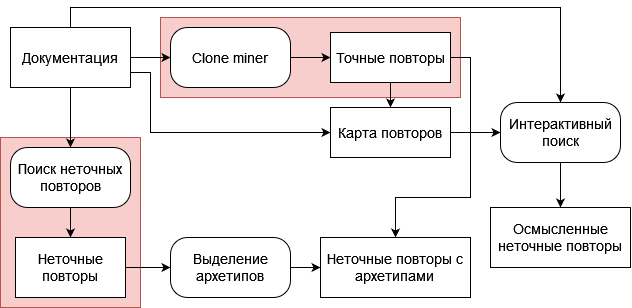
\includegraphics[scale=0.65]{pictures/DuplicateFinder.png}
	\centering
	\caption{Схема работы Duplicate Finder. Красным отмечены компоненты, которые планируется заменить}
	\label{fig:DuplicateFinder}
\end{figure}

Сам поиск повторов делится на две категории -- поиск точных и неточных повторов. В Duplicate Finder для этого используются внешние инструменты: CloneMiner \cite{bib:tool:CloneMiner} для точных повторов, FuzzyRepetitions \cite{bib:tool:FuzzySearch} и NgrammSearch \cite{bib:tool:ImprovedNgramSearch} для неточных. Механизм выглядит следующим образом: на этапе поиска повторов нужный инструмент вызывается при помощи CLI, потом результаты его работы читаются из файла, конвертируются в общий формат, и затем происходит переход на следующий этап. Далее рассмотрим недостатки такого подхода.

Основной проблемой является неоднородность компонентов для поиска. Во-первых, они написаны на разных языках -- Python, C++, C\#, что влечет за собой необходимость в дополнительных внешних зависимостях и эмуляторах. Во-вторых они абсолютно изолированы друг от друга, из-за чего возникает ряд проблем: весь процесс поиска каждый раз происходит с нуля, отсутствует возможность хранить какие-либо промежуточные состояния и т.п.

Кроме того, каждый инструмент является отдельным проектом, в связи с чем возникает проблема поддержки -  у каждого инструмента свои авторы, свой жизненный цикл. На данный момент ни один из этих проектов не поддерживается. Особенно стоит отметить проблему с CloneMiner. Это единственный инструмент для поиска точных повторов и от него зависит много функционала Duplicate Finder, однако он является закрытой разработкой и от него есть только готовые бинарники для Windows, что, очевидно, сильно мешает развитию проекта в целом.

Проблемой также является ограниченность интерфейсов этих инструментов. Каждый из них предоставляет возможность передавать набор параметров, однако их разнообразие достаточно ограниченно. Кроме того, все интерфейсы отличаются между собой и даже одни и те же настройки передаются по-разному, что вноси дополнительные неудобства в работу.

% TODO: Написать, что так то по хорошему много общего, так что можно и объединить

В таблице \ref{table:SearchTools} приведена краткая сводка об основных инструментах для поиска повторов в Duplicate Finder.

\begin{figure}[h!]
	\centering
	\include{tables/SeachTools.tex}
	\caption{Инструменты поиска повторов}
	\label{table:SearchTools}
\end{figure}

\subsection{Определение требований}
Новый механизм поиска призван устранить обозначенные выше проблемы. Для его разработки необходимо определить основные требования, реализация которых позволить добиться этой цели. Для нового инструмента поиска повторов были сформулированы следующие функциональные и нефункциональные требования:

\begin{enumerate}
	\item Инструмент должен быть написан на языке Python для бесшовной интеграции в Duplicate Finder.
	\item Должна существовать возможность поиска как точных так и неточных повторов, при этом для них должен быть единый интерфейс.
	\item Процесс поиска должен быть универсальным и различаться только в основном применяемом алгоритме.
	\item Инструмент должен иметь как API для использования в качестве библиотеки, так и CLI для внешнего использования.
	\item Должен предоставляться обширный набор параметров для настройки поиска.
\end{enumerate}

%==============================================================================
\section{Проектирование механизма поиска}

В данной главе подробно описываются логика построения основного конвеера механизма поиска, его этапы, а также алгоритмы для поиска точных и неточных повторов.

\subsection{Предобработка текста}

Сперва стоит обратить внимание на то, что основной целью механизма будет поиск повторов в документации. Документация может быть описательной или справочной, однако в обоих случаях она обычно представляет собой комбинацию текста на естественном языке и исходного кода, хоть и в различных пропорциях. Из-за этой особенности по сути ее можно воспринимать как простой текст, так как в ней отсутствует строгая структура программы. Это значит, что главным фокусом будет нахождение текстовых повторов.

При проектировании механизма в первую очередь нужно подумать про то, какие шаги приведут к наиболее оптимальному результату поиска. Так как найденные фрагменты в конечном итоге нужны пользователю для улучшения документации, чем более семантически осмысленными они будут - тем лучше. Это, означает, что для улучшения результатов необходимо сначала каким-то образом обработать текст. В данной ситуации хорошо подойдут методы NLP \cite{bib:art:NLP}, часто используемые в машинном обучении \cite{bib:art:Preprocessing}, например, в нейронный сетях \cite{bib:art:NeuralNetworks, bib:tool:NeuroDupDetect}, для работы с естественными языками. Далее перечислим основные подходы, которые можно применить при предобработке текста в механизме поиска.

\textbf{Фильтрация спецсимволов}. Тексты часто содержат большое количество специальных символов. Для естественного языка они в основном представлены пунктуацией, для исходного кода -- различные управляющие символы языка, такие как скобки и кавычки. Хотя такие символы и могут иметь некоторый семантический смысл, они выполняют вспомогательную роль и плохо отражают содержание. Кроме того, они сильно мешать поиску повторов, так как вносят значительные помехи. Поэтому первым шагом необходимо очистить текст от всех спецсимволов.

\textbf{Удаление стоп слов}. В естественных языках присутствует множество вспомогательных слов -- предлоги, частицы, артикли и т.п., которые также не относятся к содержанию. Они называются стоп слова. Такие слова часто встречаются в тексте и распределены достаточно равномерно, из-за чего они по сути являются шумом, поэтому удаление стоп слов при обработке текста является часто применяемой практикой в машинном обучении. Данный подход будет использоваться в качестве второго шага обработки.

Для поиска точных повторов предобработка включает только два шага, обозначенные выше, так как следующие шаги подразумевают трансформацию слов. Это позволяет улучшить поиск неточных повторов, однако в такой ситуации теряется смысл точного поиска.

\textbf{Лемматизация}. Так как нашей целью является поиск содержательных повторов, хорошей идеей будет избавиться от различных грамматических особенностей естественных языков. Это особенно хорошо применимо к документации, учитывая, что в исходном коде также нередко встречаются разнообразные обычные слова (названия переменных, функций, комментарии и т.п.). В этом может помочь такой процесс как лемматизация -- приведение слова к его нормальной форме. В результате применения этого подхода в тексте будет больше одинаковых слов, что увеличит качество находимых повторов.

\textbf{Стемминг}. Еще один подход, который по большей части выполняет ту же самую роль, что и лемматизация -- это стемминг. Данный процесс представляет собой выделение из слова его основу, что позволяет игнорировать грамматические особенности языка. Как и лемматизация, способствует более хорошему поиску повторов.

Также очень важную роль играет способ представления обработанного текста, так как от этого зависит, какие методы можно будет использовать. Практически везде текст разбивается на токены, которые потом используются в качестве минимальной единицей обработки. Однако, в разных инструментах используются различные структуры для представления текста. Самые распространенные -- это дерево токенов и массив токенов. Первый вариант обычно используется при работе со структурированными документами, такими как исходный код, второй -- при работе с естественными текстами, что больше подходит к нашей задаче. Таким образом, результатом этапа предобработки текста будет являться представление текста в виде массива токенов.

\subsection{Поиск точных повторов}

Поиск точных повторов подразумевает нахождение фрагментов текста, которые абсолютно идентичны друг другу. В Duplicate Finder для этого использовался CloneMiner\cite{bib:tool:CloneMiner} -- инструмент для поиска клонов в ПО. Особенностью данного инструмента является подход, основанный на последовательности токенов: в отличие от многих других средств, которые используют синтаксическое дерево программы\cite{bib:tool:ASTSearch}, CloneMiner работает с программой как с простым текстом, поэтому его можно применять вне области его предназначения.

Идею алгоритма для поиска точных повторов можно позаимствовать у CloneMiner. Хотя в работе \cite{bib:tool:CloneMiner} отсутствует полноценное описание алгоритма, лежащего в основе инструмента, а его реализация является закрытым проектом, авторы упоминают основные применяемые подходы. В частности, для поиска повторов вместо часто используемого суффиксного дерева \cite{bib:art:SuffixTree} используется суффиксный массив \cite{bib:art:SuffixArray}. Так как документация представляет собой простой текст, такой подход хорошо подойдет для нашей задачи. Изначально использование суффиксного массива подразумевает работу со строками, однако несложно обобщить работу с ним для токенов. Так как в качестве повторов нас интересуют фрагменты текста, будем рассматривать весь документ как строку, а каждый токен как ее символ. Тогда, построив суффиксный массив, можно будет сразу находить целые фрагменты текста, являющиеся точными повторами.

Суффиксный массив представляет собой последовательность индексов суффиксов строки, упорядоченных в лексиграфическом порядке. Можно заметить, что в таком случае суффиксы, начинающиеся с одинаковых подстрок, будут находиться рядом в суффиксном массиве. Так как массив содержит все суффиксы строки, таким образом можно найти все точные повторы в тексте, кроме того, они будут сразу сгруппированы. Для упрощения сравнения рядом стоящих суффиксов можно использовать вспомогательную структуру -- LCP\footnote{Longest Common Prefix -- массив наибольших общих префиксов} массив \cite{bib:art:LCPArray}, которой содержит информацию о том, какая часть соседних суффиксов совпадает. Примеры этих двух структур приведены на рис. \ref{fig:SA_LCP}

\begin{figure}[h!]
	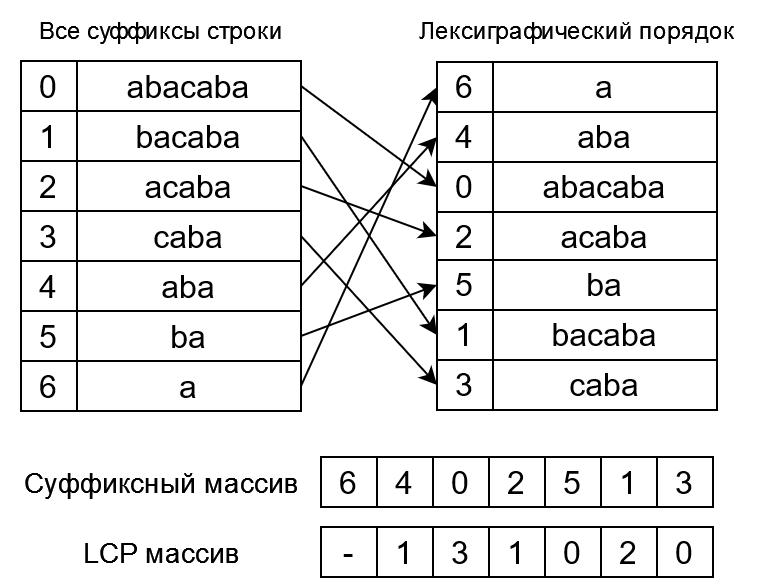
\includegraphics[scale=0.45]{pictures/SA-LCP.png}
	\centering
	\caption{Пример суффиксного и LCP массивов}
	\label{fig:SA_LCP}
\end{figure}

\textbf{Описание алгоритма}

Пусть документ представлен в виде последовательности токенов $D = [t_0,...,t_{n-1}]$. Построим для него суффиксный массив $SA = [sa_0,...,sa_{n-1}]$. Для этого можно воспользоваться Skew-алгоритмом \cite{bib:art:SkewAlg}, который позволяет построить суффиксный массив за $O(n)$ используя поразрядную сортировку (Radix sort). Такой подход хорошо подходит для нашей цели, так как минимальной единицей обработки является токен, если быть точнее -- его id, и используемый алфавит будет достаточно маленького размера. Затем построим LCP массив $L = [l_0,...,l_{n-1}]$ на основе суффиксного, что можно также сделать за $O(n)$ используя идею, описанную в \cite{bib:art:LCPArray}.

После этого будем итерироваться по суффиксному массиву. Определим параметр $m$ как минимальный размер дубликатов. Для каждого суффикса $s_i, i \in [1,n-1]$ значение $l_i$ показывает сколько общих токенов он имеет с $s_{i-1}$, и пока $l_i \ge m$ все эти фрагменты являются повторами одной группы. Когда определены все суффиксы текущей группы $[s_j,...,s_k]$, нужно проверить, являются ли суффиксами других более длинных суффиксов. Для этого каждый суффикс расширяется пока они имеют одинаковый токен слева $t_{s_j - 1} = ... = t_{s_k - 1}$. В конце алгоритма из суффиксов вырезается совпадающий префикс и создается группа точных повторов, а соответствующие токены помечаются как использованные, и далее пропускаются. Таким образом, каждый токен может быть обработан максимум один раз, из-за чего сложность алгоритма будет $O(n)$, хотя и с достаточно большой константой.


\subsection{Поиск неточных повторов}

Понятие неточных повторов можно определить различными способами. В рамках данной работы, учитывая используемые алгоритмы поиска, под группой неточных повторов будем понимать набор текстовых фрагментов $G = (g_1,...,g_n)$ такой, что для каждой пары $g_i, g_j \in G$ и некоторой функции схожести $f_{sim}$ выполняется неравенство $f_{sim}(g_i, g_j) \le T$, где $T\ge0$ -- заранее определенный параметр. Таким образом, какие фрагменты будут считаться повторами в основном зависит от выбора функции, а строгость отбора -- от параметра.

\subsubsection{Алгоритм на основе редакционного расстояния}

Одним из распространенных способов сравнения строк является редакционное расстояние или расстояние Левинштайна -- минимальное количество операций удаления, вставки и замены символов, которое необходимо для трансформирования одной строки в другую. Этот подход лежит в основе инструмента \cite{bib:tool:FuzzySearch}. Далее рассмотрим алгоритм подробнее.

Сначала весь текст, представляющий собой последовательность токенов, равномерно разбивается на фрагменты одинакового размера. Затем все фрагменты попарно сравниваются, и если два каких-либо фрагмента достаточно похожи -- они сохраняются как пара повторов. Основной функцией схожести как раз и является редакционное расстояние, исчисляемое как разница в токенах между фрагментами. Так как вычисление редакционного расстояния процесс достаточно трудоемкий, для оптимизации фрагменты сначала сравниваются по их хешам, которые рассчитываются заранее для каждого фрагмента.  Эта оценка является достаточно грубой, но помогает отсеять сильно отличающиеся пары. Граничные значения схожести являются внешними параметрами алгоритма. На последнем этапе пары повторов объединяются в группы и затем проводится расширение повторов в этих групп за счет объединения с соседними фрагментами и удаления пересечений между группами.

Хотя основную концепцию данного подхода можно оставить, у оригинального инструмента есть ряд недостатков, решив которые можно улучшить алгоритм поиска:
\begin{itemize}
	\item могут обрабатываться только документы в формате XML, что сильно сужает область применения
	\item группы составляются простым перебором пар, что неэффективно и предоставляет мало возможностей для дальнейшей обработки
	\item используемый подход хеширования достаточно ограничен и дает слишком неточную оценку
\end{itemize}

\textbf{Описание алгоритма}

Так как предобработкой текста и балансировкой групп занимаются отдельные компоненты, сосредоточим внимание на основной части алгоритма поиска. Будем рассматривать входной документ $D$ как последовательность из $n$ токенов $D = [t_0,...,t_{n-1}]$. Определим размер фрагментов $0 < m < n$ и равномерно разобьем текст на $k = n / m$ фрагментов этого размера (если $n mod m \ne 0$, тогда дополним текст с конца пустыми токенами). В результате получим набор фрагментов $[g_0,...g_{k-1}]$, где $g_i = [t_{i * m},...,t_{i * (m + 1) - 1}]$. 

После разбиения для каждого фрагмента вычислим его отпечаток в виде 32-битного хеша, используя подход sim-hash\cite{bib:art:SimHash}. Для этого посчитаем хеш каждого токена при помощи алгоритма MD5\cite{bib:art:MD5}. Выбор алгоритма хеширования обусловлен тем, что для наших целей криптографическая стойкость роли не играет, а при этом MD5 вычисляется быстрее популярной альтернативы SHA256\cite{bib:art:MD5vsSHA256}. Далее для фрагмента $g_i$ определим результирующих хеш $h_i$ на основе хешей токенов: возьмем последние 32 бита каждого из них, и для каждой позиции, если более половины битов равны одному, то в результат запишем 1, иначе 0. Укороченный пример хеширования приведен на рис. \ref{fig:Hashing}.

\begin{figure}[h!]
	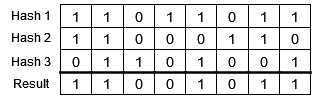
\includegraphics[scale=0.9]{pictures/Hash.png}
	\centering
	\caption{Пример вычисления итогового хеша}
	\label{fig:Hashing}
\end{figure}

Затем происходит попарное сравнение. Если разница в хешах фрагментов $g_i, g_j$, определенная как количество единиц в числе $h_i \oplus h_j$, не превышает определенной границы, то вычисляется редакционное расстояние между фрагментами. Для этого применяется алгоритм Укконена \cite{bib:art:UkkonenASM} для приблизительного сравнения строк (approximate string matching). Данный подход позволяет оптимально дать ответ на вопрос: больше ли редакционное расстояние между элементами, чем заданная граница, что мы и хотим выяснить. Так как размеры фрагментов одинаковы, а максимальное количество допустимых операций константно, сложность вычисления будет $O(m)$. Если в итоге фрагменты успешно проходят оба этапа сравнения, то они записываются, как пара повторов. В общей сложности этот этап замет не больше $O(k^2 * m) = O(\frac{n^2}{m})$

После нахождения всех пар повторов, необходимо объединить их в группы. Можно заметить, что по сути эти пары образуют неориентированный граф, где вершинами являются фрагменты, а ребра отображают их сходство. Графы очень широко распространены и имеют множество применений в разных областях, и, соответственно, существует большое количество различных алгоритмов и подходов для работы с графами, поэтому такое представление является очень выгодным. Составление групп повторов происходит путем поиска компонент связности полученного графа. Как более строгий, но медленный вариант можно использовать, например, поиск всех клик\footnote{Клика -- максимальный полный подграф} графа. Так как поиск компонент связности даже в худшем случае не будет превышать $O(c^2)$, в целом сложность алгоритма можно оценить как $O(\frac{k^2}{m})$

\subsubsection{Алгоритм на основе N-грамм}

Еще один популярный подход для работы с текстами -- это N-граммы. 

Данный алгоритм основан на идее из работы \cite{bib:tool:ImprovedNgramSearch}. Суть идеи заключается в следующем: текст разбивается на предложения, для каждого предложения вычисляется множество N-грамм. Затем предложения объединяются в группы по такому принципу: если множество N-грамм предложения-кандидата хотя бы на x\% пересекается с каждым предложением группы, то это предложение добавляется в эту группу.


\subsection{Балансировка групп повторов}

После того, как найдены основные группы повторов, можно сказать, что цель механизма поиска достигнута. Однако, можно попробовать улучшить полученные результаты. Будем пытаться сбалансировать две группы повторов путем склеивания повторов и удаления их из группы. Для того, чтобы определять, когда это надо, а когда нет, будем руководствоваться, во-первых, метриками качества(например, blow-up\cite{bib:art:JuergensCloneDetect}), и следить, чтобы они не ухудшались при балансировании, а во-вторых введем некоторую функцию значимости, и если у результирующих групп значимость больше, чем у изначальных, тогда балансируем. В результате группы будут более осмысленные.


%==============================================================================
\section{Особенности реализации}

\subsection{Используемые технологии}

\subsection{Обзор функциональности}

\subsubsection{Предобработка}

\subsubsection{Поиск повторов}

\subsection{Оптимизация}



%Сначала проводилась алгоритмическая оптимизация -- при помощи профайлера находилось узкое место программы и оптимизировались применяемые там подходы и сам код.

%Для ускорения Python'а в существует ряд технологий, самые широко используемые из которых -- это Cython, Numba, PyPy, MyPyC. Для выбора какой-то конкретного подхода необходимо сравнить, насколько хорошо каждая из данных технологий подходит для проекта в целом и какой потенциальный выигрыш в скорости может обеспечить.


%\begin{table}[ht]
%	\centering
%	\begin{tabular}{| c | c | c | c | c |}
%		\hline
%		\textbf{Название} & \textbf{Способ оптимизации} & \textbf{Сложность интеграции} & \textbf{Поддержка библиотек} & \textbf{Кроссплатформенность} \\
%		\hline 
%		Numba & Jit-компиляция & Нужно сильно подстраивать код & Слабая поддержка библиотек & Есть \\
%		\hline
%		MyPyC & Компиляция в С код & Минимальные изменения кода & Слабая поддержка библиотек & Нет \\
%		\hline
%		Cython & Компиляция в С код & Минимальные изменения кода & Слабая поддержка библиотек & Нет\\
%		\hline
%		PyPy & Jit-компиляция & Не требует изменений в коде & Поддерживает практически все библиотеки & Есть\\
%		\hline
%	\end{tabular}
%	\caption{Инструменты поиска повторов}
%	\label{table:OptimizeTools}
%\end{table}

%На основе анализа доступных технологий было принято решение использовать PyPy. 

%\begin{table}[ht]
%	\centering
%	\begin{tabular}{| c | c | c |}
%		\hline
%		\textbf{Минимальный размер повтора} & \textbf{Без оптимизации} & \textbf{С использованием PyPy} \\
%		\hline 
%		1 & 1 & 1 \\
%		\hline
%		2 & 2 & 2 \\
%		\hline
%		3 & 3 & 3 \\
%		\hline
%		4 & 4 & 4\\
%		\hline
%	\end{tabular}
%	\caption{Инструменты поиска повторов}
%	\label{table:OptimizeResults}
%\end{table}


%==============================================================================
\section{Тестирование}

Для тестирования инструмента были выбраны документации нескольких проектов: GIMP Manual, PostgreSQL Manual, Zend Framework Manual, Subversion book. Для этих документов был проведен поиск, и собрана статистика по найденным группам повторов. Результаты приведены ниже в таблицах \ref{table:StrictSearch} и \ref{table:FuzzySearch}.

\begin{table}[ht]
	\centering
	\begin{minipage}{0.9\textwidth}
\begin{adjustbox}{center}
\begin{tabular}{|l||c|c|c|c|}
	\hline
	& GIMP & PostgreSQL & Subversion & Zend Framework \\
	\hline
	\hline
	Токены & 132554 & 72728 & 110270 & 164035 \\
	\hline
	Группы повторов & 400 & 289 & 218  & 557 \\
	\hline
	Средний размер группы & 2.57 & 2.30 & 2.17 & 2.44 \\
	\hline
	Средняя длина повтора & 14.59 & 16.31 & 17.27 & 16.58 \\
	\hline
	Покрытие документа & ~11\% & ~14\% & ~7\% & ~13\% \\
	\hline
	
\end{tabular}
\end{adjustbox}
\end{minipage}
	\caption{Результаты точного поиска}
	\label{table:StrictSearch}
\end{table}

\begin{table}[ht!]
	\centering
	\begin{minipage}{0.9\textwidth}
\begin{adjustbox}{center}
\begin{tabular}{|l||m{0.15\textwidth}|m{0.15\textwidth}|m{0.15\textwidth}|m{0.2\textwidth}|}
	\hline
	Документ & Группы повторов & Средний размер группы & Средняя длина повтора & Покрытие документа \\
	\hline
	\hline
	GIMP Manual & 574 & 2.65 & 13.64 & 15\% \\
	\hline
	PostgreSQL Manual & 464 & 2.66 & 17.17 & 25\% \\
	\hline
	Subversion book & 282 & 2.27 & 18.93 & 10\% \\
	\hline
	Zend Framework guide & 522 & 2.32 & 22.96 & 16\% \\
	\hline
	Blender Manual & 1393 & 2.48 & 14.22 & 16\% \\
	\hline
	Python Requests & 23 & 2.26 & 20.16 & 28\% \\
	\hline
\end{tabular}
\end{adjustbox}
\end{minipage}
	\caption{Результаты неточного поиска}
	\label{table:FuzzySearch}
\end{table}


%==============================================================================
%% У заключения нет номера главы
% \newpage
% \[\]
\newpage
\section*{Заключение}
В ходе данной работы были получены следующие результаты.
\begin{enumerate}
   	\item Проанализированы основные подходы и средства, которые используются в существующих инструментах для поиска повторов: синтаксические и суффиксные деревья, нейронные сети, обработка естественного языка, алгоритмы хеширования, N-граммы.
   	\item Выявлены следующие основные требования к новому механизму поиска: объединение точного и неточного поиска, унификация процесса поиска, высокая степень настраиваемости.
   	\item Спроектирован конвейер для механизма поиска, состоящий из трех основных этапов: предобработка текста, применение алгоритмов поиска повторов, балансировка групп повторов.
   	\item Разработаны алгоритмы для точного и неточного поиска повторов на основе использованных в Duplicate Finder инструментов
   	\item Выполнена реализация инструмента на языке Python с использованием пакета NLTK для предобработки текста, исходный код доступен по ссылке \mbox{\url{https://github.com/IceWind2/TextDuplicateSearch}}; проведена интеграция с Duplicate Finder.
   	\item Проведено тестирование инструмента на корпусе документов, по результатам работы собрана статистика и проведен ее анализ.
\end{enumerate}

%==============================================================================

\setmonofont[Mapping=tex-text]{CMU Typewriter Text}
\bibliographystyle{ugost2008ls}
\bibliography{diploma}
\end{document}
